%%
%% Author: lukas
%% 27.12.2018
%%

% Preamble
\documentclass[12pt]{article}
\usepackage[DIV=12]{typearea}
\usepackage[utf8]{inputenc}
\usepackage[czech]{babel}
\usepackage{graphicx}
\usepackage{subcaption}
\usepackage{float}
\usepackage{enumitem}
\usepackage{amsmath}
\usepackage{amssymb}
\usepackage{caption}
\usepackage{blkarray}
\usepackage{mathtools}
\usepackage{array}
\usepackage{bm}
\usepackage[T1]{fontenc}
\usepackage{amsfonts}


% Document
\begin{document}

    \title{Lineární programování}
    \author{Lukáš Forst}
    \maketitle

    \section{Definice úlohy LP}\label{sec:definice-úlohy-lp}
    Ze zadání máme
    \begin{align*}
        min & \sum_{t=0}^{N-1}f(u(t))\\
        f(a) &= \left
        \{ \begin{array}{ll}
               |a| & |a|\leq 1\\
               2|a|-1 & |a| >1
        \end{array} \right.
    \end{align*}
    $min \sum_{t=0}^{N-1}f(u(t))$  převedeme do LP tvar s využitím podmínek pro $f(a)$.\\
    Následující výraz bude mít tedy stejnou minimální hodnotu jako původní za zadání
    \begin{align*}
        \text{min} \enspace & 1^T z,\enspace z \in \mathbb{R}^N\\
        \text{za podmínek} \enspace & z_t \geq u_t\\
        &z_t  \geq -u_t\\
        &z_t  \geq 2u_t-1\\
        &z_t  \geq -2u_t-1
    \end{align*}
    Tento výraz můžeme pomocí slackových proměnných a rozložením \(u_t\) na rozdíl dvou kladných čísel převést na
    rovnosti s proměnnými většími než 0
    \begin{align*}
        \text{min} \enspace 1^T z,\enspace z \in \mathbb{R}^N\\
        \text{za podmínek} \enspace z_t - u_t^+ + u_t^- - s_{t1} &= 0\\
        z_t + u_t^+ - u_t^- - s_{t2} &= 0\\
        z_t - 2u_t^+ + 2u_t^- - s_{t3} &= -1\\
        z_t + 2u_t^+ - 2u_t^- - s_{t4} &= -1
    \end{align*}
    Nyní převedeme na LP i výraz
    \begin{align*}
        x(t+1) = Ax(t) +bu(t), \enspace t = 0,\ldots,N-1
    \end{align*}
    Výraz si nejprve rozepíšeme po prvcích
    \begin{align*}
        \left[\begin{array}{c}
                  x_{t+1,1}\\
                  \vdots\\
                  x_{t+1,n}
        \end{array}\right] =
        \left[\begin{array}{c c c}
                  a_{1,1}& \ldots &a_{1,n}\\
                  &\vdots&\\
                  a_{n,1}& \ldots &a_{n,n}
        \end{array}\right]
        \left[\begin{array}{c}
                  x_{t,1}\\
                  \vdots\\
                  x_{t,n}
        \end{array}\right]+
        \left[\begin{array}{c}
                  b_{1}\\
                  \vdots\\
                  b_{n}
        \end{array}\right] u(t), \enspace t = 0,\ldots,N-1
    \end{align*}
    Rovnici pro libovolný prvek můžeme zapsat jako
    \begin{align*}
        x_{t+1,i} &= a_{i,1}x_{t,1}+\ldots + a_{i,n}x_{t,n} + b_{i}u_t\\
        \text{kde}\enspace t &= 0\dots N-1\\
        i &= 0\dots n
    \end{align*}
    Kde pro \(t = 0\) je \(x_0\) vektor konstant.
    Pokud \(t=N-1\) pak je \(x_{t+1}\) také vektor konstant.\\
    Opět rozložíme všechny proměnné na rozdíl nezáporných čísel
    \begin{align*}
        x_{1,i}^+ - x_{1,i}^- - b_{i}u_0^+ + b_{i}u_0^- &= a_{i,1}x_{0,1}+\dots + a_{i,n}x_{0,n} \\
        x_{t+1,i}^+ - x_{t+1,i}^- - b_{t,i}u_t^+ + b_{t,i}u_t^- - Ax_t&= 0 \qquad \text{kde} \quad t = 1\dots N-2 \\
        - Ax_{N-1} - b_{N-1,i}u_t^+ + b_{N-1,i}u_{N-1}^-&= -x_{N,i}
    \end{align*}
    Kde
    \begin{align*}
        Ax_t = a_{i,1}x_{t,1}^+ - a_{i,1}x_{t,1}^- +\dots + a_{i,n}x_{t,n}^+ - a_{i,n}x_{t,n}^-
    \end{align*}
    Nyní výše zmíněné rovnice můžeme vzít a vložit do jednoho zápisu pro LP program $min\{c^T x| Ax = b, x \geq 0\}$. \\
    Parametry z originálního zadání jsou následující
    \begin{align*}
        A = \begin{bmatrix}
                1 & 1\\
                0 & 0.95
        \end{bmatrix}, \enspace
        b = \begin{bmatrix}
                0 \\
                0.1
        \end{bmatrix}, \enspace
        x(0) = (0,0), \enspace
        x_{des} = (10,0), \enspace
        \text{ze zadání } \bm{a)} \enspace N = 2
    \end{align*}
    Tedy naše matice budou vypadad následovně (některé vektory jsem transponoval pro lepší čitelnost) \\
    Výraz, který minimalizujeme $c^T x$
    \begin{align*}
        c^T &=
        \left[\setlength\arraycolsep{6pt}
        \begin{array}{*{18}{c}}
            1 & 1 & 0 & 0 & 0 & 0 & 0 & 0 & 0 & 0 & 0 & 0 & 0 & 0 & 0 & 0 & 0 & 0
        \end{array}
        \right] \\
        x^T &= \left[\setlength\arraycolsep{1pt}
        \begin{array}{*{18}{c}}
            z_1 &z_2 &s_{1,1} &s_{1,2} &s_{1,3} &s_{1,4} &s_{2,1} &s_{2,2} &s_{2,3} &s_{2,4} &u_{1}^+ &u_{1}^-
            &u_{2}^+ &u_{2}^- &x_{1,1}^+ &x_{1,1}^- &x_{1,2}^+ &x_{1,2}^-
        \end{array}
        \right]
    \end{align*}
    Kde pro indexy $c^T$ platí
    \begin{align*}
        c_1, c_2 = z\\
        c_3 \dots c_{10} = s \\
        c_{11} \dots c_{14} = u \\
        c_{15} \dots c_{18} = x
    \end{align*}
    A podmínka $Ax = b$
    \begin{align*}
        b^T &= \left[
        \begin{array}{*{18}{c}}
            0 & 0 & -1 & -1 & 0 & 0 & -1 & -1 & 0 & 0 & -10 & 0
        \end{array}
        \right] \\
        x^T &= \left[\setlength\arraycolsep{3pt}
        \begin{array}{*{18}{c}}
            z_1 &z_2 &s_{1,1} &s_{1,2} &s_{1,3} &s_{1,4} &s_{2,1} &s_{2,2} &s_{2,3} &s_{2,4} &u_{1}^+ &u_{1}^-
            &u_{2}^+ &u_{2}^- &x_{1,1}^+ &x_{1,1}^- &x_{1,2}^+ &x_{1,2}^-
        \end{array}
        \right] \\
        A &=
        \left[ \setlength\arraycolsep{2.5pt}
        \begin{array}{*{18}{c}}
            1 &0 &-1 &0 &0 &0 &0 &0 &0 &0 &-1 &1 &0 &0 &0 &0 &0 &0\\
            1 &0 &0 &-1 &0 &0 &0 &0 &0 &0 &1 &-1 &0 &0 &0 &0 &0 &0\\
            1 &0 &0 &0 &-1 &0 &0 &0 &0 &0 &-2 &2 &0 &0 &0 &0 &0 &0\\
            1 &0 &0 &0 &0 &-1 &0 &0 &0 &0 &2 &-2 &0 &0 &0 &0 &0 &0\\
            0 &1 &0 &0 &0 &0 &-1 &0 &0 &0 &0 &0 &-1 &1 &0 &0 &0 &0\\
            0 &1 &0 &0 &0 &0 &0 &-1 &0 &0 &0 &0 &1 &-1 &0 &0 &0 &0\\
            0 &1 &0 &0 &0 &0 &0 &0 &-1 &0 &0 &0 &-2 &2 &0 &0 &0 &0\\
            0 &1 &0 &0 &0 &0 &0 &0 &0 &-1 &0 &0 &2 &-2 &0 &0 &0 &0\\
            0 &0 &0 &0 &0 &0 &0 &0 &0 &0 &0 &0 &0 &0 &1 &-1 &0 &0\\
            0 &0 &0 &0 &0 &0 &0 &0 &0 &0 &-0.1 &0.1 &0 &0 &0 &0 &1 &-1\\
            0 &0 &0 &0 &0 &0 &0 &0 &0 &0 &0 &0 &0 &0 &-1 &1 &-1 &1\\
            0 &0 &0 &0 &0 &0 &0 &0 &0 &0 &0 &0 &-0.1 &0.1 &0 &0 &-0.95 &0.95
        \end{array}
        \right]
    \end{align*}
    Kde pro indexy $b^T$ platí
    \begin{align*}
        b_{1} \dots b_{8} = \text{pravá strana } \mathbf{z} \text{ rovnic} \\
        b_{8} \dots b_{12} = \text{pravá strana } \mathbf{u} \text{ rovnic} \\
    \end{align*}
    \section{Grafy obsahující závislosti a optimální hodnota F}\label{sec:grafy-obsahující-závislosti-a-optimální-hodnota-f}
    Pro hodnoty
    \begin{align*}
        A = \begin{bmatrix}
                1 & 1\\
                0 & 0.95
        \end{bmatrix}, \enspace
        b = \begin{bmatrix}
                0 \\
                0.1
        \end{bmatrix}, \enspace
        x(0) = (0,0), \enspace
        x_{des} = (10,0), \enspace
        N = 20
    \end{align*}
    nalezla moje implementace řešení
    \begin{align*}
        F = 15.9119
    \end{align*}
    Grafy zobrazující závislosti $u(t), x_1(t), x_2(t)$ na $t$ pak vypadají takto
    \begin{figure}[h!]
        \centering
        \begin{subfigure}[b]{0.5\linewidth}
            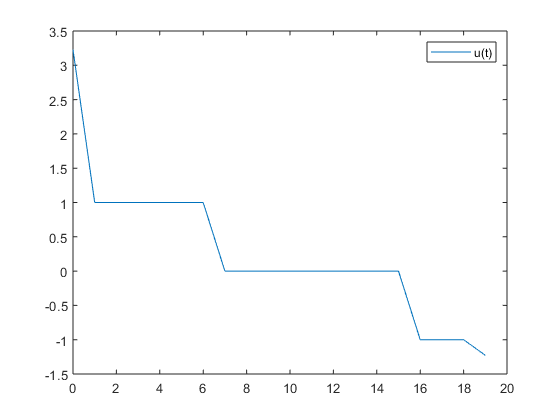
\includegraphics[width=\linewidth]{ut_t.png}
            \caption{Závislost $u(t)$ na $t$}
        \end{subfigure}
        \begin{subfigure}[b]{0.5\linewidth}
            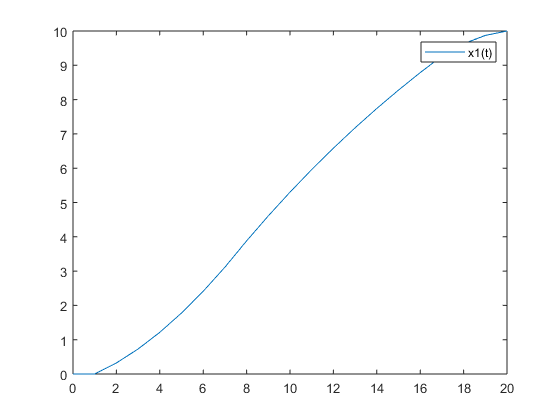
\includegraphics[width=\linewidth]{x1_t.png}
            \caption{Závislost $x_{1}(t)$ na $t$}
        \end{subfigure}
        \begin{subfigure}[b]{0.5\linewidth}
            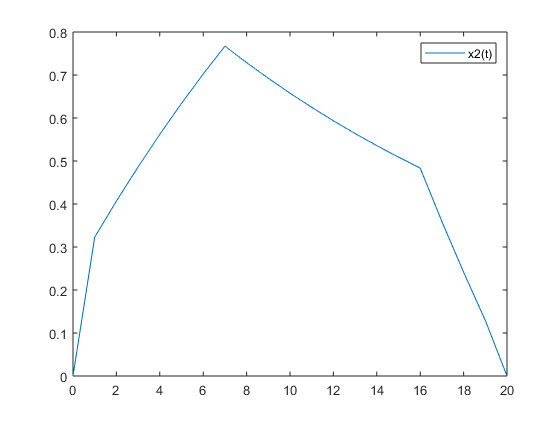
\includegraphics[width=\linewidth]{x2_t.png}
            \caption{Závislost $x_{2}(t)$ na $t$}
        \end{subfigure}
        \caption{Grafy závislostí $u(t), x_1(t), x_2(t)$ na $t$}
    \end{figure}
\end{document}